\documentclass{beamer}
\usepackage{hyperref}
\setbeamertemplate{theorems}[numbered]
\setbeamertemplate{footline}[frame number]
\renewcommand{\matrix}[2]{ \left(\begin{array}{#1} #2 \end{array}\right)}
%../../../papers/PJTpreamble.tex
\begin{document}

\title{INFINITESIMAL PHASE RESPONSE CURVES FOR PIECEWISE SMOOTH DYNAMICAL SYSTEMS}
%\subtitle{Subtitle}
\author % (optional, for multiple authors)
{Youngmin Park\inst{1}\\
Committee chair: Peter J. Thomas\inst{1}\\
Committee members: Hillel J. Chiel\inst{2}, Alethea Barbaro\inst{1}, Michael G. Hurley\inst{1}}
\institute % (optional)
{
  \inst{1}%
  Department of Mathematics
  \inst{2}%
  Department of Biology
  
  Case Western Reserve University
}
\frame{\titlepage}


% 
% \begin{frame}\frametitle{PJT comments}
% \begin{enumerate}
% \tiny
%\item Motivation: 1. Biological Oscillators. 2. (why) Phase Response Curves (matter) (and note the iPRC cannot be solved for analytically except in a few cases, which you should be familiar with; use Morris Lecar as an example of one you cannot find analytically). 3. Piecewise linear flows arise in several contexts: Glass networks, Coombes/McKean model,  Shaw et al's ``iris model", which is a piecewise linear analog of the ``sine'' SHC system, which in turn is motivated by influence of passage near a fixed point on response of limit cycle to perturbations.  

% 2: the motivation for PRC from a general biological level is OK -- many process in nature are cyclic, including motions produced by animals.  An active area of research in mathematical bio is in trying to understand how animals control their own movements.  At a general level, how do you incorporate information from the world to how you're moving. Mathematically the form that rhythmic systems take tend to involve a limit cycle (period orbit that nearby solutions converge to it; isolated (non-Hamiltonian), periodic orbit). typically use stable limit cycles in modeling CPGs (interested in modeling CPGS can be modeled using stable LC).

% john gukenheimer 1980 isochrons and phaseless sets (...math. biol.) -- information on isochrons

%once w ehave a LC, how do we quantify effects of perturbations -- can label points in BA by where they arrive at the LC (isochrons).  In iPRCs we assume perturbations are weak. We end up speeding it up or slowing it down => directional derivate

%The ongoing context for this work involves how sensitive the system is to perturbations (patterned inputs from body)

% typically ODE's are smooth, but don't have to be for LC's.

% focus on the PRC as quickly as possible -- develop as clearly and succinctly as possible.

%\item Put results on PWL flows and the adjoint before discussing the kink in the iris system and iPRC in arc length?  You can mention that the peak sensitivity lies in at the boundary and in a similar locus for the sine SHC, but we don't really have a complete answer as to why that is.  The PWL adjoint solution is much more complete at this point.
%\item You can talk about the kink and also the iPRC via arc length for Morris-Lecar at the end, under ``future work".
%\item ``biological motivation slide": motivation is to understand how response of a limit cycle trajectory to external perturbations changes when the LC passes near a fixed point.  The origin of this question is in thinking about how one incorporates proprioceptive feedback to modulate the tempo of a CPG.  But for the MS thesis the focus should be more on the mathematical questions that result.  You can certainly mention \textit{Aplysia} (since Prof. Chiel will be there!) but not make it a focus, I think.
%\item To define phase, 1. introduce a deterministic ODE system with smooth right hand side; 2. introduce a limit cycle and its basin of attraction; 3. introduce the isochron or phase function in this context.  You can't just jump in with "the phase of a limit cycle is a number..."  The phase function is a map from the underlying point space (the basin of attraction of the LC, which is some open subset of $\mathbb{R}^2$ for the ML system) to the circle $\mathcal{S}^1$, parametrized as $\theta(x)\in[0,1)$.
%\item the iPRC is \emph{defined} as a derivative -- it is the directional derivative of $\theta(x)$ in the direction of the perturbation.  (not quite ``The iPRC is equivalent to the gradient of the isochron function over a limit cycle.'') Then you should give the argument for why it satisfies the adjoint equation.
%\item You can introduce the models earlier in the introduction section, provided you explain why each is relevant to the discussion.  And break them up, and show a picture for each.  The pictures can come from Shaw et al provided you cite.
%\item slide 11: does the iris iPRC resemble ML or does it resemble the sine system?
%\item iPRC and arc length: we have numerical results but no theory.  skip this part until there is a theory.  We can discuss your two Lemmas, but I don't think the story is there yet?  You can come back to it, but put the strongest part of the story first, to allay any concerns in the committee over the substance of the thesis.
%\item The start of the PWL section looks good so far.  It would help a lot to have one big diagram with everything labeled, something like what's in my notes.  
% \end{enumerate}
% \normalsize
% \end{frame}

\begin{frame}
\frametitle{Table of Contents}
\tableofcontents%[currentsection]
\end{frame}

\section{Introduction}
\subsection{Motivation}

\begin{frame}
  \frametitle{\insertsection}
  \framesubtitle{\insertsubsection}

  \begin{itemize}
  \item Biological oscillators
  \item Phase response curves
  \item Piecewise linear flows
  \begin{itemize}
  \item Gene regulatory (Glass) networks
  \item Piecewise linear neuronal models (Coombes 2008\cite{Coombes:2008:SIADS})
  \item Iris system (Shaw et al. 2012)%, a piecewise linear analog of the sine SHC system.
  \end{itemize}
  \end{itemize}

  %\item Interested in the underlying structure of the feeding mechanism in \textit{Aplysia Californica}
  %	\begin{itemize}
  %	\item A special case of a central pattern generator (CPG)
  %	\end{itemize}
  %\item The results of Shaw et al. (2012) are the results of theoretical perturbative analysis on candidate models for the feeding mechanism.
\end{frame}
  
\subsection{The phase response curve}

\begin{frame}
\frametitle{\insertsection}
  \framesubtitle{\insertsubsection}
  Consider a deterministic system of ODEs in $\mathbb{R}^n$:
  \begin{equation}
  \frac{dx}{dt} = F(x),
  \end{equation}

  where $F$ is a smooth map $F:\mathbb{R}^n \rightarrow \mathbb{R}^n$. Let the system have a solution $\gamma$, which represents an isolated periodic orbit with period $T$,
  \begin{equation}
  \gamma(t) = \gamma(t+T), \quad \forall t \in \mathbb{R}^+,
  \end{equation}

  such that nearby solutions converge to it as $t \rightarrow \infty$.  We call this a \underline{stable limit cycle}.  Note: the set of initial conditions that converge to the limit cycle is called the basin of attraction (B.A.).
\end{frame}


\begin{frame}

  \begin{definition} The \underline{phase} of a limit cycle with period $T$ is a function $\theta: \gamma \rightarrow S^1$ with $S^1$ parameterized as $\theta(\gamma(t)) \in [0,1)$ and
  \begin{equation}
  \frac{d }{dt}\left (\theta(\gamma(t)) \right ) = 1/T,
  \end{equation}
  \end{definition}
  where $\theta = 0$ is chosen arbitrarily.
\end{frame}

\begin{frame}
   \begin{figure}
   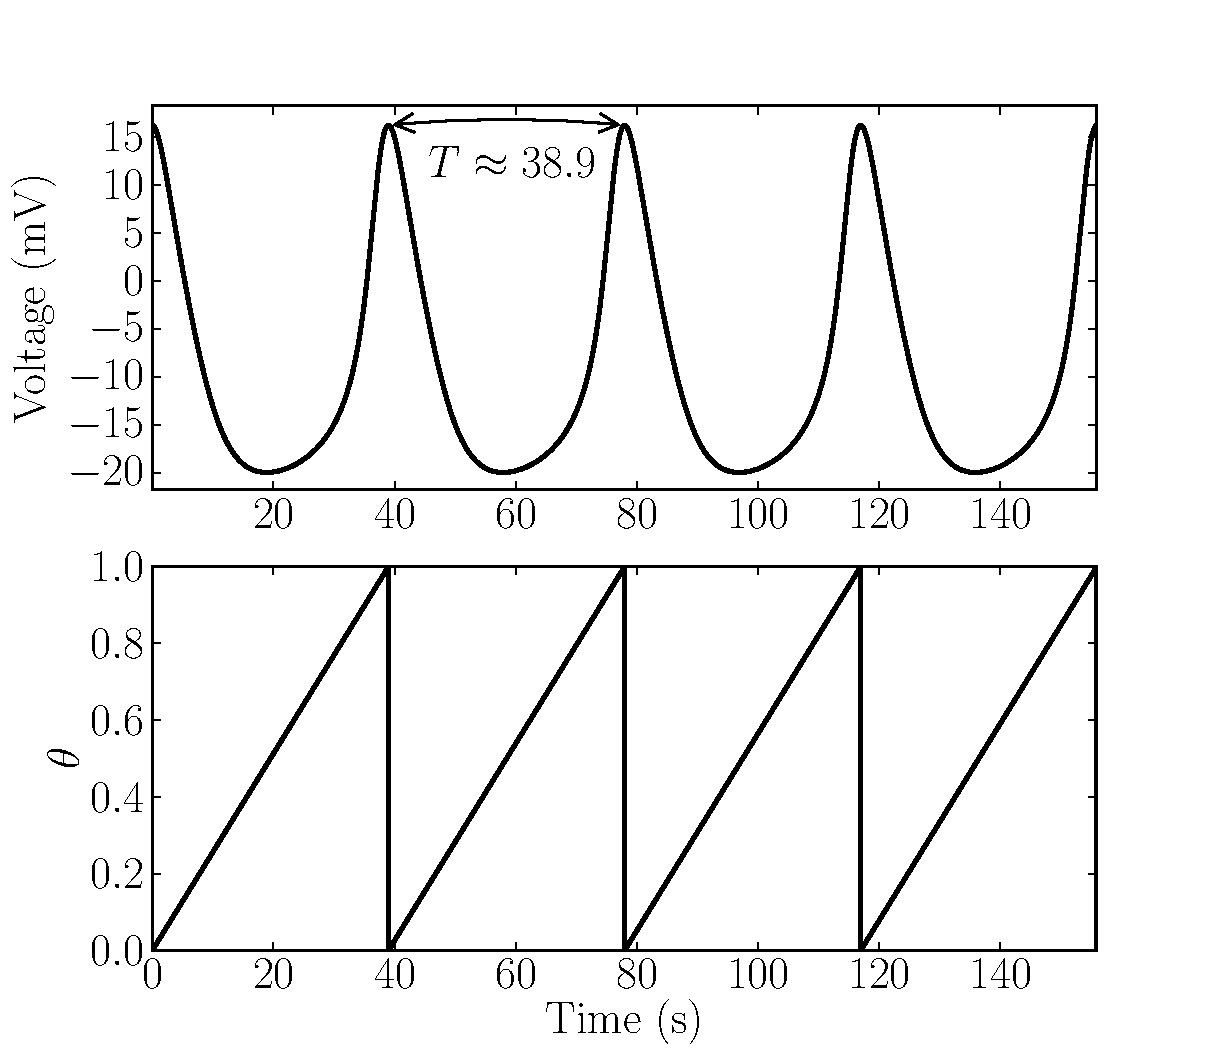
\includegraphics[width=\textwidth]{dthetadt_fig.pdf}
  \end{figure}
\end{frame}


  \begin{frame}
    \begin{definition}
  Given a point $x_0 \in B.A.$, there exists a unique $\theta(x_0)$ such that 
  \begin{equation}
    \lim_{t \rightarrow \infty} | x(t) - \gamma(t + T\theta(x_0))  | \rightarrow 0,
  \end{equation}
  
  The value $\theta(x_0)$ is the \underline{asymptotic phase} of the point $x_0$.

  \end{definition}

  \begin{definition}
  An \underline{isochron} is a level curve of the phase function $\theta$, consisting of points that share the same asymptotic phase.
  
%   For a trajectory $x(t)$ with initial condition $x_0 \in BA$, there exists a unique $\theta(x_0)$ such that
%   \begin{equation}
%     \lim_{t \rightarrow \infty} | x(t) - \gamma(t + T\theta(x_0))  | \rightarrow 0,
%   \end{equation}
%   
%   then these points are on the same isochron. 
  \end{definition}
   Note: all points on the isochron share the same asymptotic phase, so $\forall x \in B.A.$,
  \begin{equation}
   \frac{d\theta(x)}{dt} = 1/T.
  \end{equation}
  
  \end{frame}
  
  \begin{frame}
  \begin{figure}
   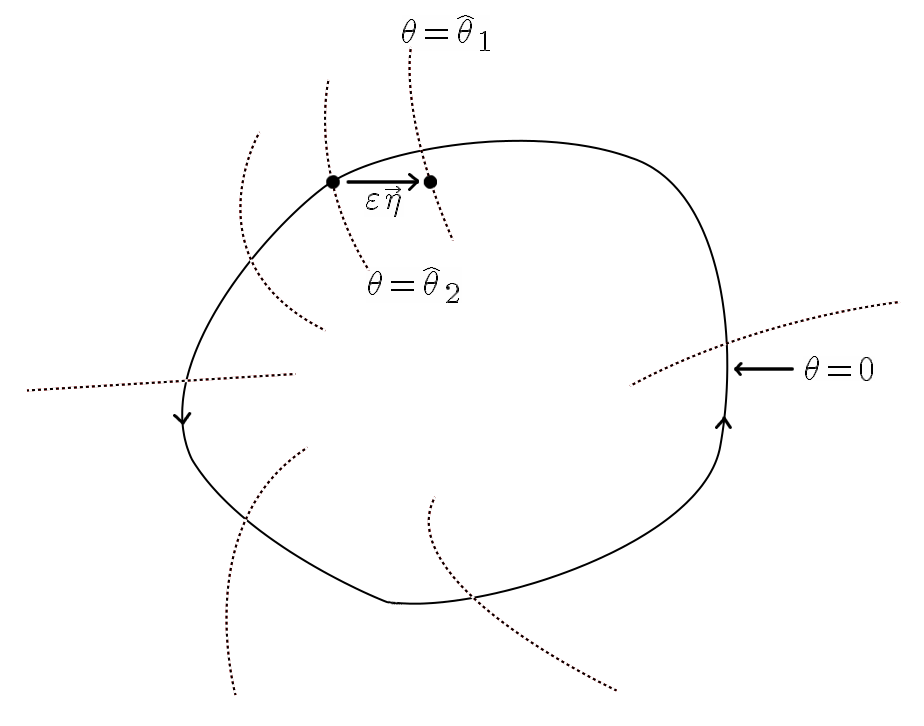
\includegraphics[width=\textwidth]{isochron-demo.png}
  \end{figure}

   
  \end{frame}

  
\begin{frame}
Suppose we perturb a limit cycle with a perturbation of size $\varepsilon$ in the unit vector direction $\eta$.  How does the asymptotic phase of the perturbed trajectory compare to the phase of the unperturbed trajectory?

\begin{equation}
\theta(\gamma(t) + \varepsilon \eta) = \theta(\gamma(t)) + \varepsilon D\theta(\gamma(t))\cdot \eta + O(\varepsilon^2).
\end{equation}

\begin{equation}
\Delta \theta = \theta(\gamma(t) + \varepsilon \eta) - \theta(\gamma(t)) = \varepsilon D\theta(\gamma(t))\cdot \eta + O(\varepsilon^2).
\end{equation}

\begin{equation}
\lim_{\varepsilon \rightarrow 0} \frac{\Delta \theta}{\varepsilon} = D\theta(\gamma(t))\cdot \eta =: z(t) \cdot \eta
\end{equation}

\begin{itemize}
 \item An explicit expression for $z(t)$ exists for a small number of cases.
\end{itemize}
\end{frame}


% \begin{frame}
% One way to solve for the iPRC is by using the adjoint equation.  The linearization about the limit cycle $\gamma$ satisfies the equation
% \begin{equation}
%  \frac{dy}{dt} = DF(\gamma(t)) y(t),
% \end{equation}
% 
% where $y(t)$ is an arbitrary, small perturbation.
% \begin{equation}
% \begin{split}
%  0 &= \frac{d}{dt} (z(t)\cdot y(t))\\
%  &=\frac{dz}{dt}\cdot y(t) +z(t)\cdot\frac{dy}{dt}\\
%  &=\frac{dz}{dt}\cdot y(t) +z(t)\cdot DF(\gamma(t)) y(t)\\
%  &=\frac{dz}{dt}\cdot y(t) +DF(\gamma(t))^T z(t) \cdot y(t)\\
%  &=\left [ \frac{dz}{dt} +DF(\gamma(t))^T z(t)\right ] y(t).
%  \end{split}
% \end{equation}
% \end{frame}

  \begin{frame}
 \frametitle{\insertsection}
    	\framesubtitle{\insertsubsection}
    \begin{figure}
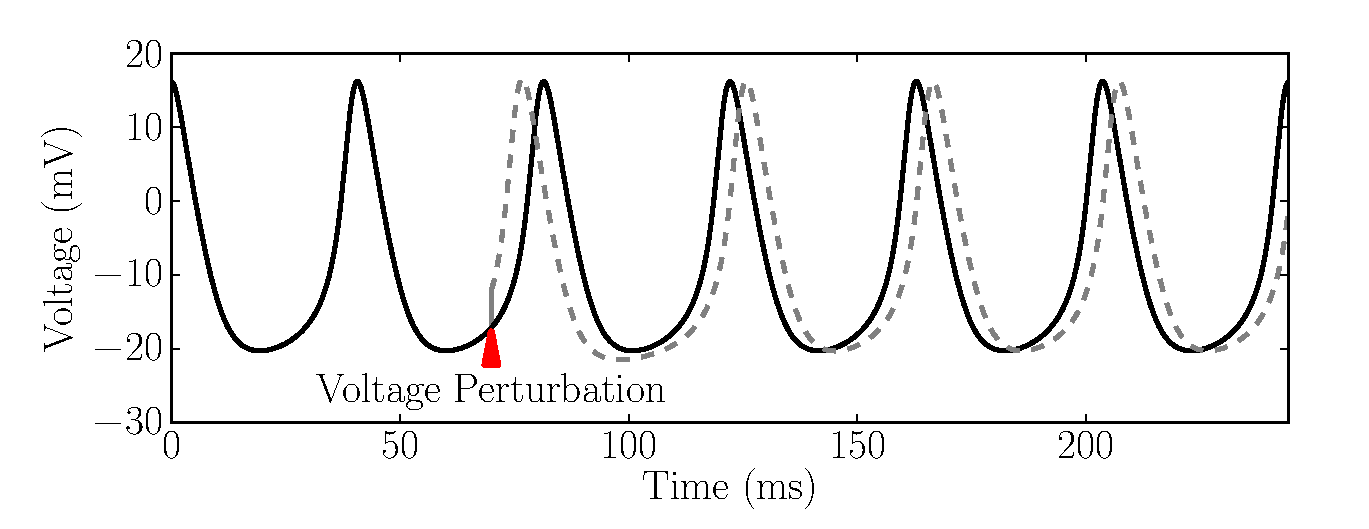
\includegraphics[width=1\textwidth]{voltage-pert-ml-vt.pdf}
\caption{Example of a phase response for the Morris-Lecar model: a voltage perturbation at phase $\phi \approx .6$ ($t \approx 70ms$) of a limit cycle leads to a change in timing of $\Delta \theta \approx .1$.  }
\end{figure}
  \end{frame}

  \begin{frame}
 \frametitle{\insertsection}
    	\framesubtitle{\insertsubsection}
    \begin{figure}
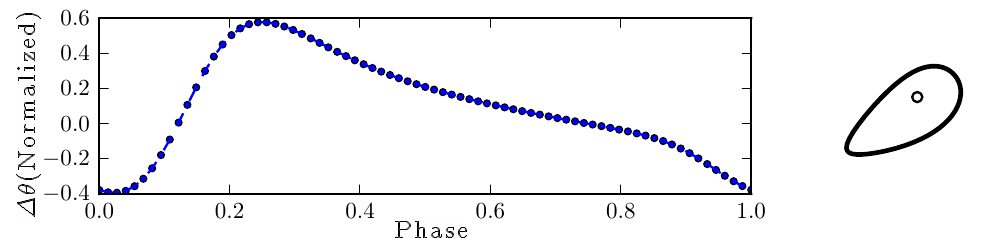
\includegraphics[width=1\textwidth]{voltage-pert-ml-quarter.png}
\caption{Example of an iPRC: Blue dots indicate the phase at which we apply an infinitesimal perturbation of size 1e-4 to the same model. The resulting phase difference is shown along the vertical axis.  The voltage-time plot from the last slide is now shown in a phase space representation on the right (Shaw et al. 2012).}
\end{figure}
  \end{frame}



\begin{frame}
 The iPRC, $z(t)$, satisfies the adjoint equation
\begin{equation}
 \frac{dz}{dt} = -DF(\gamma(t))^T z(t).
\end{equation}

 Provides an alternative method to calculating the iPRC.

\end{frame}


\subsection{Assumptions for planar piecewise smooth dynamical systems}
\begin{frame}
\frametitle{\insertsection}
  \framesubtitle{\insertsubsection}

   By piecewise smooth differential equations, we mean the following: Let $B \subset \mathbb{R}^n$.  A vector field $F:B \rightarrow \mathbb{R}^n$ is piecewise smooth on $B$ if there exists a finite number of open sets such that
   \begin{enumerate}
    \item $B_i \cap B_j = \varnothing, \forall i \neq j$
    \item $B \subset \bigcup_{k=1}^K \bar{B}_k$
    \item There exist smooth vector fields $F^k: \bar{B}_k \rightarrow \mathbb{R}^n$ such that  for all $x$ in $B_k$, $F^k(x)=F(x)$, 
  \end{enumerate}
  where $||F|| < \infty$ and there is a limit cycle.
\end{frame}


\begin{frame}
\begin{figure}
\frametitle{\insertsection}
  \framesubtitle{\insertsubsection}
 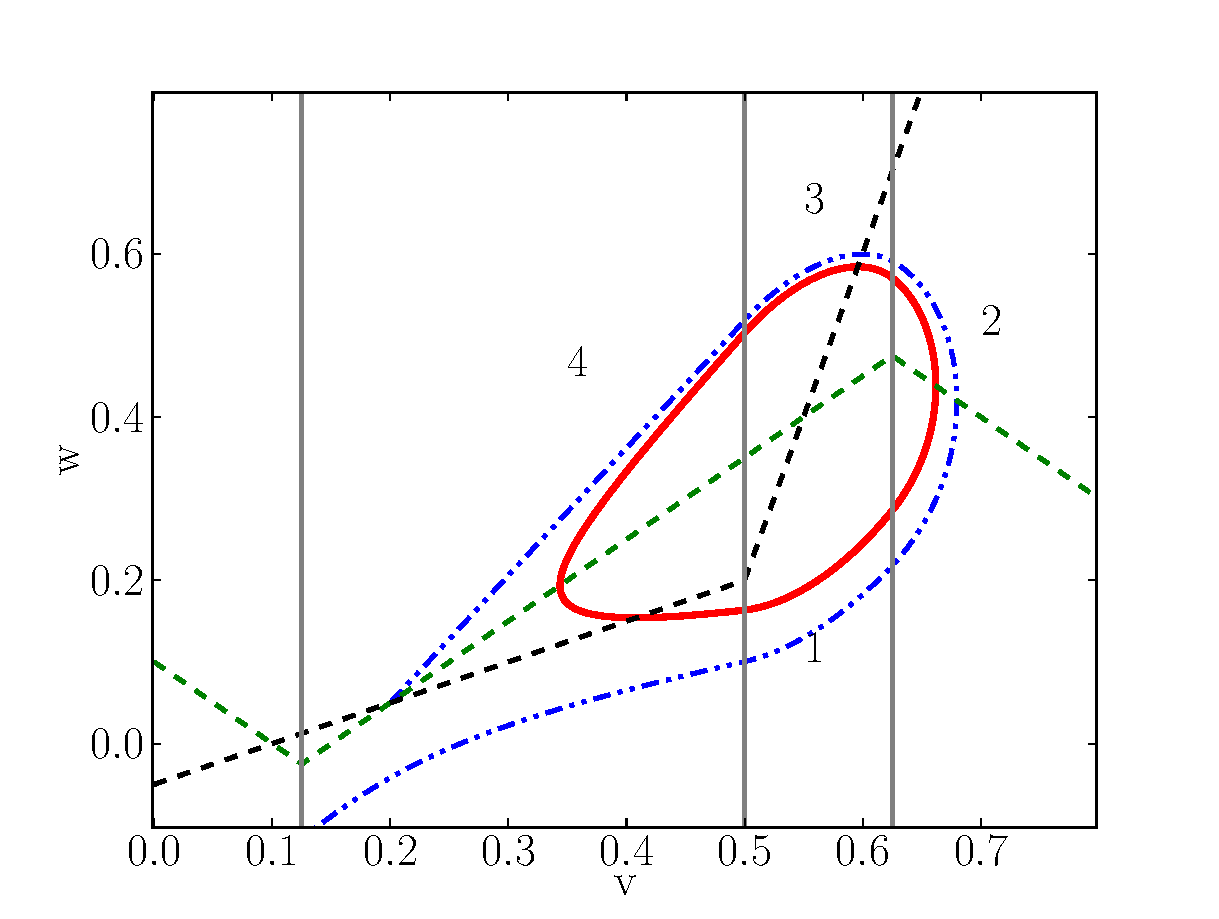
\includegraphics[width=.8\textwidth]{pml_fig.pdf}
 \caption{Example of a piecewise linear differential equation: Piecewise Morris-Lecar model (Coombes 2008).}
\end{figure}
\end{frame}

\begin{frame}
 \begin{figure}
 \frametitle{\insertsection}
  \framesubtitle{\insertsubsection}
  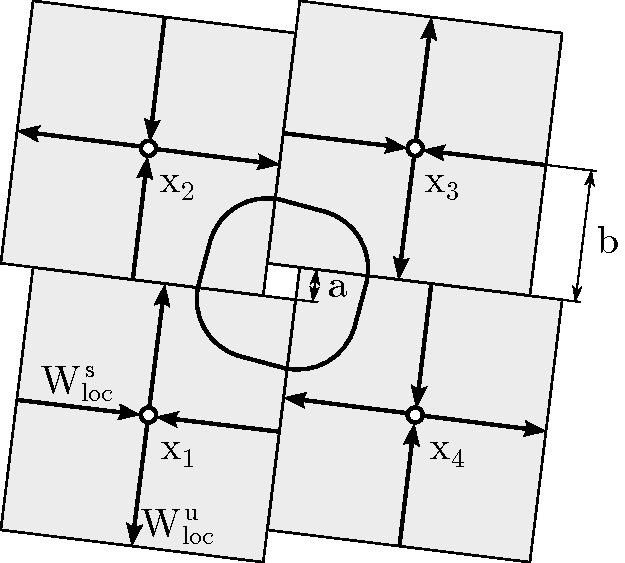
\includegraphics[width=.5\textwidth]{sine_to_iris_fig_sketch_iris.pdf}
  \caption{Example of a piecewise linear differential equation: Iris system.  Figure due to Kendrick Shaw (Shaw et al. 2012) \cite{ShawParkChielThomas2012SIADS}.}
 \end{figure}
\end{frame}


\begin{frame}
  For piecewise smooth dynamical systems, we assume the following without proof:
  \begin{enumerate}
\item \textit{Existence and uniqueness holds for trajectories in the piecewise smooth dynamical systems we consider.}
 
 \item \textit{The system has a stable limit cycle with well-defined phase.}
 
 \item \textit{A unique asymptotic phase exists for all points in the basin of attraction.}
 
 \item \textit{Isochrons exist, are continuous and}
 
\begin{equation}
\frac{d\theta(x(t))}{dt} = 1/T, \quad \forall x(t) \in B.A.
\end{equation}
 
 \item \textit{$\theta(x)$ is differentiable in the direction tangent to the boundary.}
  \end{enumerate}
\end{frame}

\begin{frame}
 \begin{figure}
 \frametitle{\insertsection}
  \framesubtitle{\insertsubsection}
  \includegraphics[width=.6\textwidth]{iris_isochron_fig-revised.pdf}
  \caption{Isochrons of the iris system.  Figure due to Kendrick Shaw (Shaw et al. 2012).}
 \end{figure}
\end{frame}


\begin{frame}
\begin{itemize}

\item Recall the adjoint equation,
\begin{equation}
 \frac{dz}{dt} = -DF(\gamma(t))^T z(t).
\end{equation}
In general, the adjoint equation is not directly solvable for piecewise smooth systems.

\item The gradient definition,
\begin{equation}
 \lim_{\varepsilon \rightarrow 0} \frac{\Delta \theta}{\varepsilon} = D\theta(\gamma(t))\cdot \eta =: z(t) \cdot \eta,
\end{equation}
Is invalid for up to a finite number of times.

\item However, the iPRC exists and is well-defined, though it may be discontinuous.

\item We derive a general method for solving the iPRC for general planar piecewise smooth systems that allows for the use of the adjoint equation.
\end{itemize}
\end{frame}



\section{Solving the adjoint equation over boundaries of PWL systems}
\begin{frame}
\frametitle{Table of Contents}
\tableofcontents[currentsection]
\end{frame}



\subsection{General equation for discontinuous jumps across boundaries of planar systems}
  \begin{frame}
 \frametitle{\insertsection}
 \framesubtitle{\insertsubsection}
We fix notation and define terms before introducing the theorem. Let $F^R$ denote a planar vector field of a region $R$, where each region is numbered according to the direction of flow.  Given a limit cycle $\gamma = \gamma^1 + \gamma^2 +...+\gamma^K$ with period $T = t_1 +...+t_K$, we denote the final and initial values of a vector field along the limit cycle as
\begin{equation}
\begin{split}
F^R_f &= F^R(\gamma^R(t_R)),\\
F^{R+1}_0 &= F^{R+1}(\gamma^{R+1}(0)),
\end{split}
\end{equation}
where time (t) is local and $t_R$ denotes the time of flight through region R.  Let
\begin{equation}
 F^{R} = (f^{R}, g^{R}).
\end{equation}



  \end{frame}
  
% \begin{frame}
% \frametitle{\insertsection}
% \framesubtitle{\insertsubsection}
% An equivalent solution to the perturbative derivation of the iPRC uses the adjoint equation.  The solution to the adjoint equation,
% 
% \begin{equation}
%  \frac{dz}{dt} = -\left[ DF^R(\gamma(t)) \right ]^T z(t),
% \end{equation}
% 
% for over the limit cycle $\gamma$ is the iPRC.  The iPRC may also be defined by the gradient of the phase function,
% 
% \begin{equation}
%  z(t) \equiv \nabla \theta(\gamma(t)).
% \end{equation}
% 
% \end{frame}
  
  \begin{frame}
  \frametitle{\insertsection}
   \framesubtitle{\insertsubsection}
   Recall the adjoint equation (valid on the interior of each domain $R$),
   \begin{equation}
    \frac{dz^R}{dt} = A^R z(t)^R.
   \end{equation}

    Let
    \begin{itemize}
     \item $\hat{n} = (\cos\psi_R, \sin\psi_R)$ denote the vector normal to the limit cycle at a smooth boundary and $\hat{w} = (-\sin\psi_R, \cos\psi_R)$ denote the vector tangent to the boundary at the same limit cycle crossing.
     \item $z_f^R=\lim_{t\to t_R^-}z^R(t)$ be the solution to the adjoint equation at the end of region R.
     \item $z_0^{R+1}=\lim_{t\to 0^+}z^{R+1}(t)$ be the solution after the jump induced by the boundary. 
    \end{itemize}
  \end{frame}

  \begin{frame}
   \frametitle{\insertsection}
   \framesubtitle{\insertsubsection}
\begin{theorem} Let $\gamma$ be a piecewise smooth limit cycle in $\mathbb{R}^2$ satisfying assumptions $1-5$.  The iPRC for $\gamma$ satisfies the following boundary condition at the boundary $\partial^{R/R+1}$,
 \begin{equation}
z_0^{R+1}=M^R z_f^R,
\end{equation}
where
\begin{equation}
M^R = \matrix{cc}{f_0^{R+1} & g_0^{R+1}\\
-\sin\psi_R & \cos\psi_R}^{-1}\matrix{cc}{f_f^R & g_f^R\\
-\sin\psi_R & \cos\psi_R}.
\end{equation}
Existence of the required matrix inverse is guaranteed by the transverse flow condition, $F_0^{R+1}\cdot \hat{n} > 0$.
\label{theorem}
\end{theorem}
\end{frame}


\subsection{Proof}
\begin{frame}
\frametitle{\insertsection}
\framesubtitle{\insertsubsection}
\textit{Proof} Let $k \in \{ R, R+1 \}$.  By the use of the chain rule, we have the useful relation valid in the interior of each domain,
\begin{equation}
 \frac{d\theta}{dt}=F^k(x^k(t))\cdot\nabla\theta^k(x^k(t)).
\end{equation}

Recall: $d\theta/dt = 1/T$ over all regions and boundaries.  Therefore,

\begin{equation}\label{eq:thetaflow}
F_0^{R+1}\cdot z_0^{R+1}=F_f^{R}\cdot z_f^{R}=\frac{1}{T}.
\end{equation}
\end{frame}


% \begin{frame}
% \frametitle{\insertsection}
% \framesubtitle{\insertsubsection}
% Next, consider the isochron over the boundary.
%     \begin{definition} An \underline{isochron} is the set of points that have the same asymptotic phase.  Suppose $\gamma(t)$ is a stable limit cycle with period T.  Then for each point $x$ in the basin of attraction of $\gamma$ there exists a unique phase $\theta(x)$ such that 
% \begin{equation}
% \lim_{t \rightarrow \infty} | x(t) - \gamma(t + T\theta(x))| = 0,
% \end{equation}
% where $x(t)$ is a trajectory of a dynamical system with $x(0) = x$.
% \end{definition}
% The iPRC is equivalent to the gradient of the isochron function over a limit cycle.
% \end{frame}


\begin{frame}
\frametitle{\insertsection}
\framesubtitle{\insertsubsection}
The asymptotic phase function $\theta^R(x)$ is continuous along the boundary with respect to space, by assumption.

Let the interval $(w_{min},w_{max})$ lie in the basin of attraction, with $w_0=0$ the crossing point of the limit cycle.  Then for each isochron,
\begin{equation}
\theta^{R+1}(w) = \theta^R(w).
\end{equation}
\end{frame}

\begin{frame}
\frametitle{\insertsection}
\framesubtitle{\insertsubsection}
Moreover, $\theta(w)$ is differentiable in the direction of the coordinate $w$ (tangent to the boundary), so
\begin{equation}
\left(\nabla\theta^{R+1}(w)\right)\cdot\hat{w}=\left(\nabla\theta^R(w)\right)\cdot\hat{w}.
\end{equation}

In particular, for $w = 0$,
\begin{equation}
 z_0^{R+1}\cdot\hat{w}=z_f^{R}\cdot\hat{w}.
\end{equation}
\end{frame}


\begin{frame}
\frametitle{\insertsection}
\framesubtitle{\insertsubsection}
Given the equations 
\begin{equation}
\begin{split}
 F_0^{R+1}\cdot z_0^{R+1}&=F_f^{R}\cdot z_f^{R},\\
 \hat{w}\cdot z_0^{R+1}&=\hat{w}\cdot z_f^{R},
\end{split}
\end{equation}

invoke the definitions to form an expression for $z_0^{R+1}$ in terms of $z_f^{R}$.
\begin{eqnarray}
\matrix{cc}{f_0^{R+1} & g_0^{R+1}\\ -\sin\psi_R & \cos\psi_R}z_0^{R+1}
&=&
\matrix{cc}{f_f^R & g_f^R\\ -\sin\psi_R & \cos\psi_R}z_f^R,
\end{eqnarray}

Left multiplying by the inverse of the matrix on the left completes the proof. $\Box$
\end{frame}

\begin{frame}
\begin{corollary}
With the assumptions of Theorem \ref{theorem} and affine linear vector fields $F^k$, the initial condition of the iPRC, $z(t)$, must satisfy
 \begin{equation}\label{eq:eigenvalue}
z^1_0=B z^1_0,
\end{equation}
where
\begin{equation}
B=M^{K}e^{A^{K}t_K}\cdots M^1e^{A^1 t_1},
\end{equation}
$t_k$ is the time of flight through the $k^{th}$ region, $e^{A^{k}}$ is the matrix exponential of $A^k = -\left(DF^k\right)^\intercal$.  Eq.~\eqref{eq:eigenvalue} and the normalization condition,
 \begin{equation}\label{eq:normalization}
F_0^1\cdot z^1_0=\frac{1}{T},
\end{equation}
yield a unique solution for the initial condition, $z_0^1 \in \mathbb{R}^2$.
\label{corl:circuit}\end{corollary}
\end{frame}


\begin{frame}
 \frametitle{\insertsection}
\framesubtitle{\insertsubsection}
 \begin{corollary}\label{corl:c0-vector-fields}
 Under the assumptions of Corollary \ref{corl:circuit}, if adjacent vector fields evaluated along the limit cycle, $F_f^R$ and $F_0^{R+1}$, are continuous at the boundary $\partial^{R/R+1}$, then the matrix $M^R$ is the identity.
\end{corollary}
\end{frame}


\subsection{Application to piecewise linear dynamical systems}

\begin{frame}
\frametitle{\insertsection}
\framesubtitle{\insertsubsection}
Piecewise Morris-Lecar.
\begin{equation}
 \begin{split}
  C \dot{v} &= f(v) - w + I,\\
  \dot{w} &= g(v,w),
 \end{split}
\label{eq:coombes-eqs}\end{equation}

 \begin{equation}
 \begin{split}
  f(v) = \left \{ \begin{array}{ll} -v,& \quad v< a/2  \\ v - a, & \quad a/2 \leq v \leq (1+a)/2 \\ 1- v, & \quad v >(1+a)/2 \end{array} \right . ,
 \end{split}
\end{equation}

 \begin{displaymath}
   g(v,w) = \left\{
     \begin{array}{lr}
       (v-\gamma_1w+b^*\gamma_1-b)/\gamma_1, \quad v < b\\
       (v-\gamma_2w+b^* \gamma_2-b)/\gamma_2. \quad v \geq b
     \end{array}
   \right.
\end{displaymath}
\end{frame}


\begin{frame}
\begin{figure}
\frametitle{\insertsection}
  \framesubtitle{\insertsubsection}
 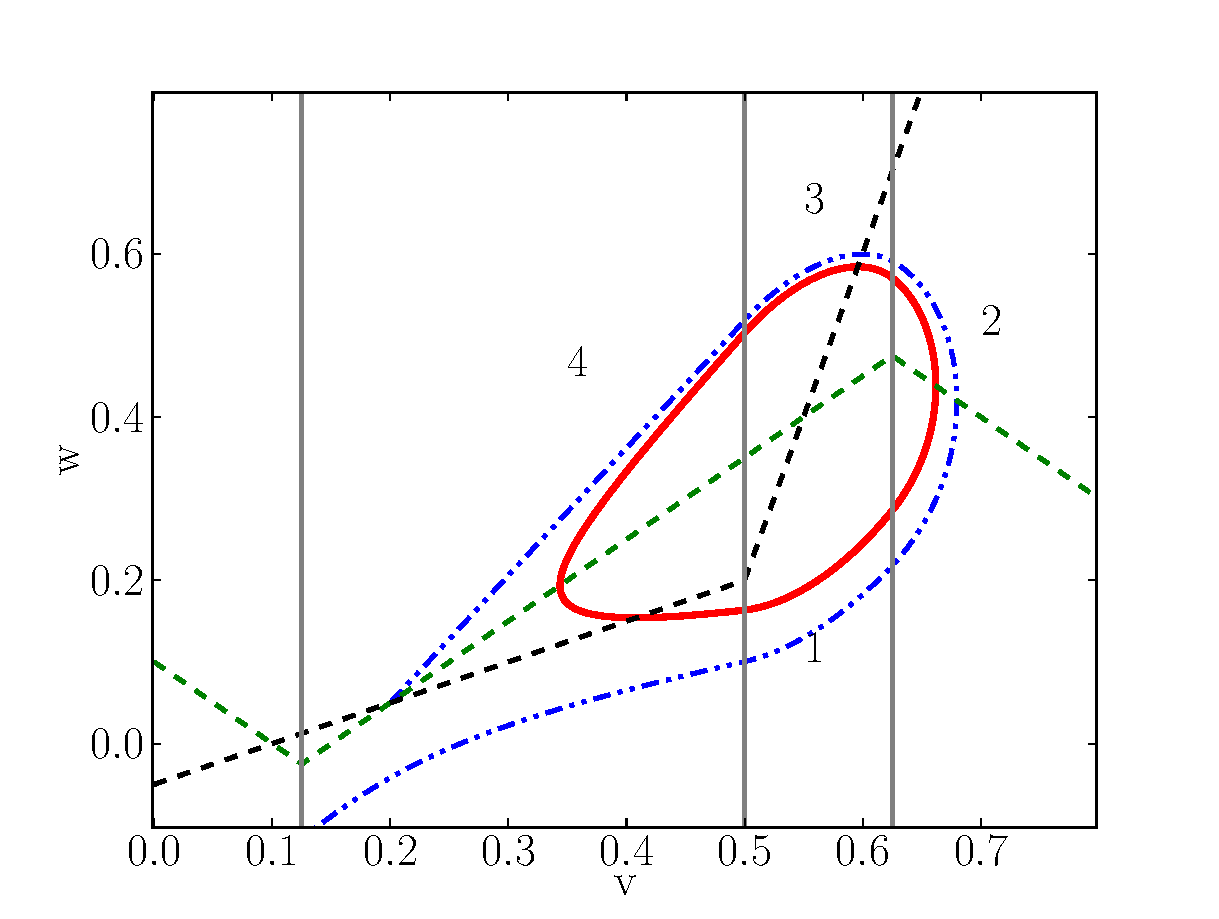
\includegraphics[width=.8\textwidth]{pml_fig.pdf}
 \caption{Piecewise Morris-Lecar model (Coombes 2008).}
\end{figure}
\end{frame}

\begin{frame}
At the boundary $v=b$, the first component of the vector field does not change, but the second component changes.  However,
 \begin{equation}
\begin{split}
g^4(b,w) - g^1(b,w) &= (-\gamma_1w+b^*\gamma_1)/\gamma_1- (-\gamma_2w+b^* \gamma_2)/\gamma_2 \\
&= 0.
\end{split}
\end{equation}

\begin{figure}
 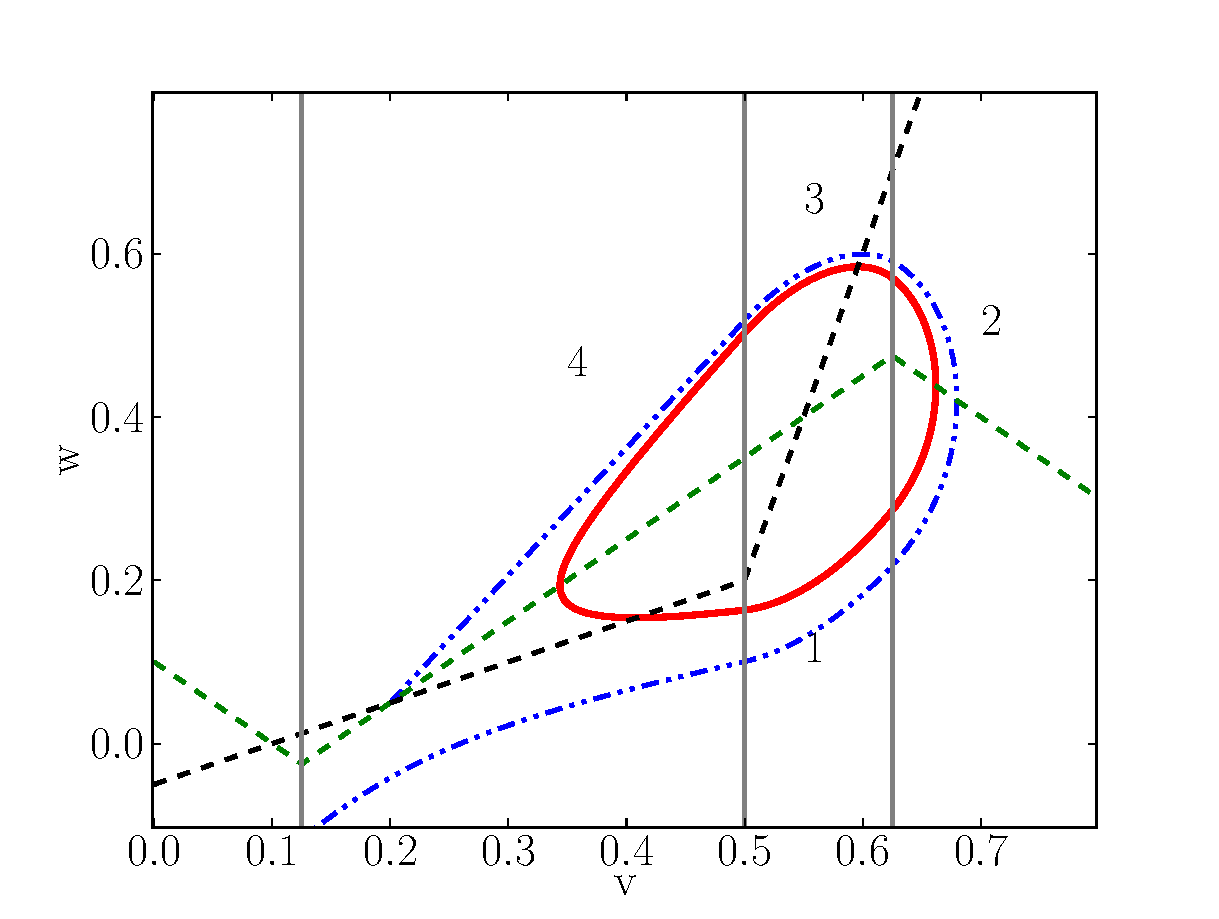
\includegraphics[width=.6\textwidth]{pml_fig.pdf}
 \caption{Piecewise Morris-Lecar model (Coombes 2008).}
\end{figure}
\end{frame}

\begin{frame}
 \begin{figure}[h!]
\begin{center} 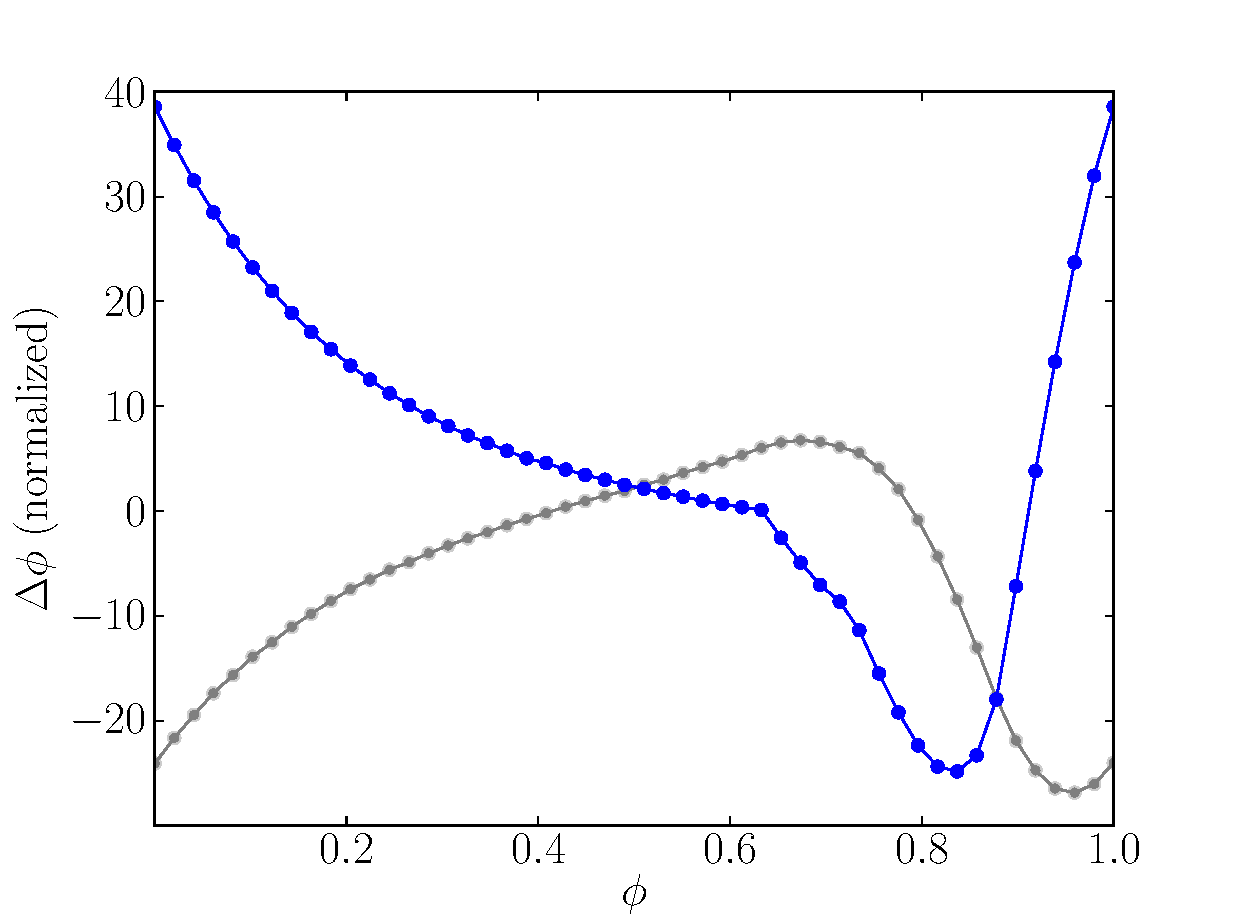
\includegraphics[width=.75\textwidth]{pml_prc_fig.pdf}\end{center}
\caption[Numerical iPRCs of the PML system]{Numerical iPRCs of the PML system. Blue: perturbations in the positive horizontal direction. Gray: perturbations in the positive vertical direction.  There are no discontinuities in either iPRC. Copyright~\copyright~~2008 Society for Industrial and Applied Mathematics.  Reprinted with permission.  All rights reserved.}
\label{fig:pml_iprc}\end{figure}
\end{frame}

\begin{frame}
 \begin{figure}
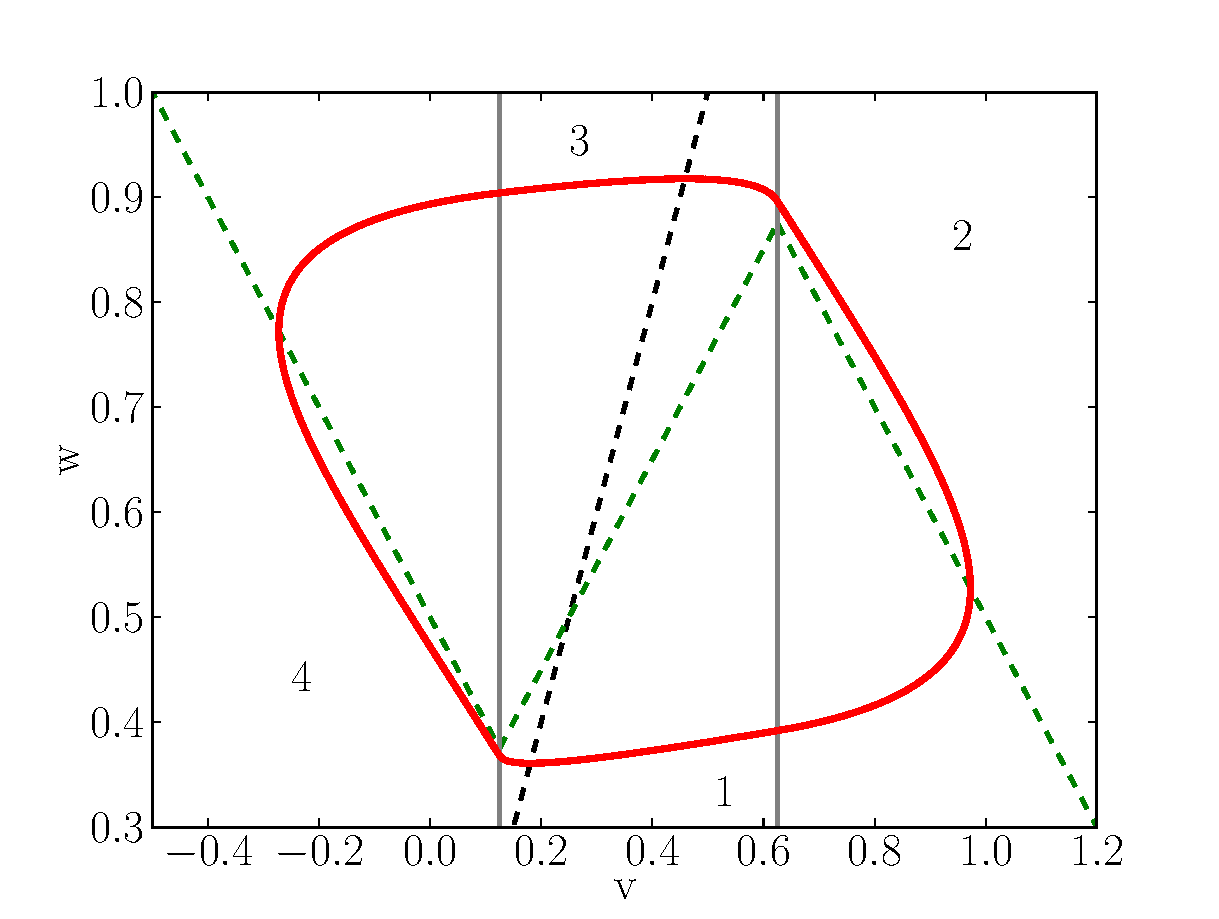
\includegraphics[width=\textwidth]{pmk_fig.pdf}
\caption{McKean Model (Coombes 2008)}\end{figure}
\end{frame}

\begin{figure}[h!]
\begin{center} 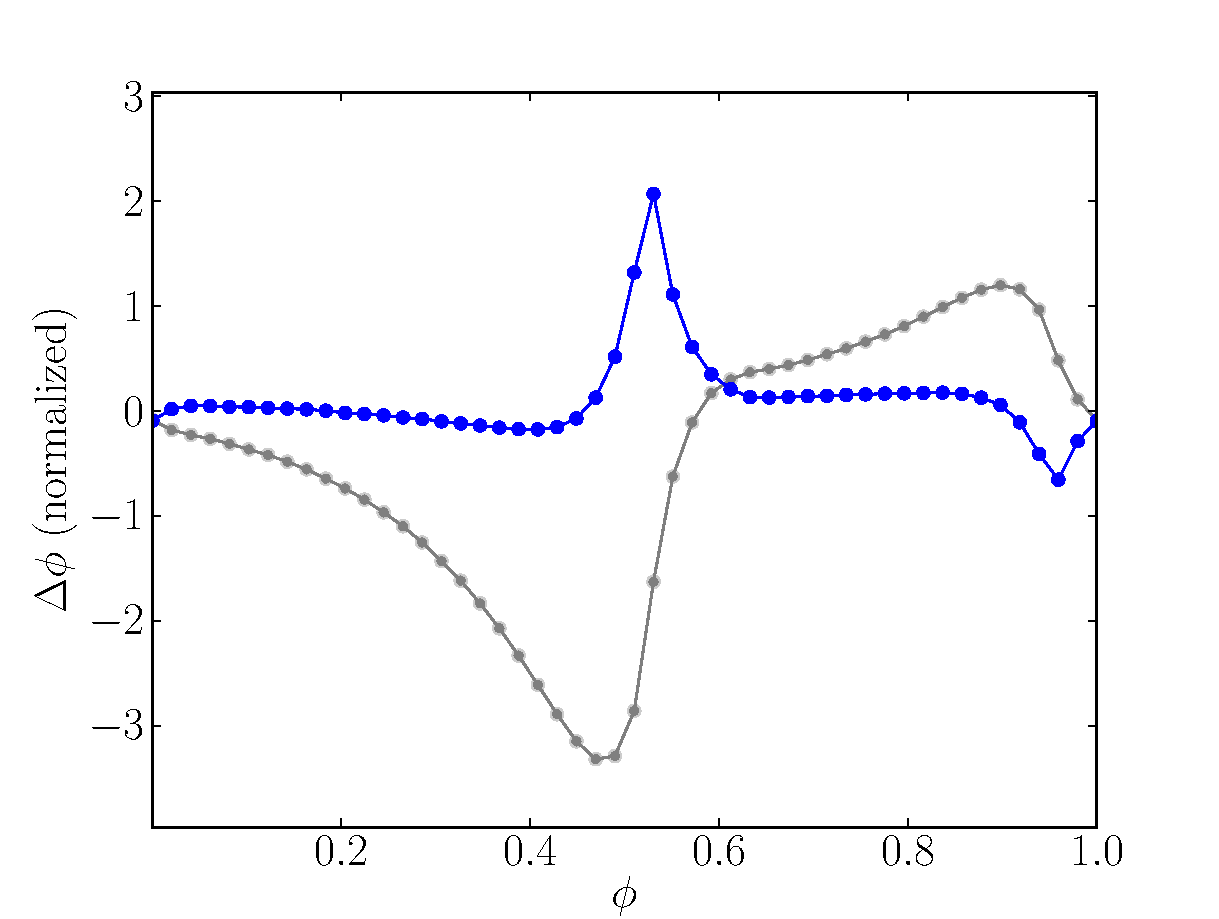
\includegraphics[width=.75\textwidth]{pmk_prc_fig.pdf}\end{center}
\caption[Numerical iPRCs of the McKean model]{Numerical iPRCs of the McKean model. Blue: perturbations in the positive horizontal direction. Gray: perturbations in the positive vertical direction.  There are no discontinuities in either iPRC. Copyright~\copyright ~2008 Society for Industrial and Applied Mathematics.  Reprinted with permission.  All rights reserved.}
\label{fig:pmk_iprc}\end{figure}


\begin{frame}
\frametitle{\insertsection}
\framesubtitle{\insertsubsection}
Iris system.

Recall the matrix $B$ of the first corollary,
 \begin{equation}
z^1_0=B z^1_0,
\end{equation}
where
\begin{equation}
B=M^{K}e^{A^{K}t_K}\cdots M^1e^{A^1 t_1},
\end{equation}
$t_k$ is the time of flight through the $k^{th}$ region, $e^{A^{k}}$ is the matrix exponential of $A^k = -\left(DF^k\right)^\intercal$.  

\end{frame}

\begin{frame}
 \frametitle{\insertsection}
\framesubtitle{\insertsubsection}
For the iris system, 
\begin{equation}
\begin{split}
 z_0^{SW} &= B z_0^{SW}\\
 &= \matrix{cc}{\frac{e^{(\lambda-1)T}}{\lambda} - e^{2\lambda T} \left ( \frac{u}{\lambda} + s \right )^2, & \frac{e^{(\lambda-1)T}}{\lambda}\left ( \frac{u}{\lambda} + s \right )\\
 e^{2\lambda T} \left ( -\frac{u}{\lambda} -s \right), & \frac{e^{(\lambda -1)T}}{\lambda}}^2 z_0^{SW}.
 \end{split}
\end{equation}
The matrix $B$ has an eigenvector $z_0^{SW} = (s,1)^T$.
\end{frame}

\begin{frame}
 \frametitle{\insertsection}
\framesubtitle{\insertsubsection}
The normalization condition,
\begin{equation}
 F_0^{SW}\cdot z^{SW}_0=\frac{1}{T},
\end{equation}
gives us the magnitude of $z_0^{SW}$.  Note that $F_0^{SW} = (-\lambda, u)$, so
\begin{equation}
\begin{split}
 F_0^{SW}\cdot z^{SW}_0 &= -\lambda s + u\\
 & = -\lambda u^\lambda + u.
\end{split}
\end{equation}
In order for $z_0^{SW}$ to satisfy the normalization condition, it must be scaled by $\frac{1}{T(-\lambda u^\lambda + u)}$.
\end{frame}

\begin{frame}
 Therefore, the initial condition of the adjoint equation is
 \begin{equation}
  z_0^{SW} = \left (\frac{s}{T(-\lambda u^\lambda + u)},\frac{1}{T(-\lambda u^\lambda + u)} \right )^T.
 \end{equation}
 Recalling that $t = \theta T = \theta \log(1/u)$,
\begin{equation}
\begin{split}
 z^{SW}(t) &= \matrix{cc}{e^{\lambda t} & 0 \\ 0 & e^{-t}}z_0^{SW}\\
 & = \matrix{cc}{e^{\lambda \theta T} & 0 \\ 0 & e^{-\theta T}} \matrix{c}{  \frac{u^\lambda}{T(u-\lambda u^\lambda)} \\ \frac{1}{T(u-\lambda u^\lambda)}  }\\
 & = \matrix{c}{  \frac{u^{\lambda(1-\theta)}}{T(u-\lambda u^\lambda)} \\ \frac{u^\theta}{T(u-\lambda u^\lambda)}  }.
\end{split}
\end{equation}

 
\end{frame}

\section{Conclusions}
\begin{frame}
 \frametitle{\insertsection}
 \begin{enumerate}
 \item The infinitesimal phase response curve (iPRC) for a limit cycle in a smooth system satisfies an adjoint equation, but this approach is not directly applicable to piecewise smooth dynamical systems.

 \item I presented a method for handling discontinuities in a vector field, that extends the adjoint equation approach to piecewise smooth dynamical systems.

 \item My method allows for the efficient derivation of exact iPRCs, in the special case of piecewise linear dynamical systems.
\end{enumerate}

\end{frame}



\begin{frame}[allowframebreaks]
        \frametitle{References}
        \bibliographystyle{plain}
        \bibliography{math,PJT}
\end{frame}



\begin{frame}
\frametitle{Acknowledgements}
Thanks to Dr. Peter J. Thomas, Dr. Hillel J. Chiel, Kendrick Shaw\footnote{MD/PhD at Case Western Reserve Medical School}, and the other committee members, Dr. Alethea Barbaro and Dr. Michael Hurley.
\end{frame}

\begin{frame}
\frametitle{iPRCs of Normal Forms}
The iPRC of the normal form of a saddle-node-on-invariant circle (SNIC) bifurcation is proportional to (Ermentrout 1996 \cite{Ermentrout1996NeuralComput})
\begin{equation}
z(\theta) \propto 1-\cos(\theta).
\end{equation}

The iPRC for models close to supercritical Hopf bifurcations may be approximated by a pure sinusoid (Brown et al. 2004, Izhikevich 2007) \cite{BrownMoehlisHolmes:2004:NeComp,Izhikevich2007}).
\begin{equation}
z(\theta) \propto \sin(\theta).
\end{equation}
\end{frame}

\begin{frame}
 \frametitle{Derivation of Adjoint Equation}
 \begin{equation}
\begin{split}
 0 &= \frac{d}{dt}\left(\frac{d\theta}{dt} \right)\\
 &=\frac{d}{dt}\left(\nabla\theta(x(t)) \cdot \frac{dx}{dt} \right)\\
 &=\left(\frac{d}{dt}\nabla\theta(x(t))\right) \frac{dx}{dt} + \nabla\theta\cdot\left(DF(x(t)) \frac{dx}{dt}\right)\\
 &=\left(\frac{d}{dt}\nabla\theta(x(t))\right) \frac{dx}{dt} + DF^T(x(t)) \cdot\nabla\theta  \frac{dx}{dt}\\
 &=\left [ \frac{d}{dt} \nabla \theta(x(t)) + DF^T(x(t))\cdot\nabla\theta(x(t)) \right ] \cdot F(x(t)).
\end{split}
\end{equation}
\end{frame}

\begin{frame}
 \frametitle{Chain Rule Applied to $d\theta/dt$}
 \begin{equation}
\begin{split}
 \frac{d\theta}{dt} &= \frac{\partial \theta}{\partial x_1}\frac{d x_1}{dt} + ... + \frac{\partial \theta}{\partial x_n}\frac{d x_n}{dt}\\
 &=\left (\frac{\partial \theta}{\partial x_1}, ..., \frac{\partial \theta}{\partial x_n} \right ) \cdot \left ( \frac{d x_1}{dt}, ..., \frac{d x_n}{dt}\right )\\
 &= \nabla \theta \cdot \frac{dx}{dt}
\end{split}
\end{equation}
\end{frame}




\end{document}